\documentclass[10pt,letter,english]{article}

\usepackage{amsmath}
\usepackage{amscd}
\usepackage{amssymb}

\usepackage{tikz}
\usetikzlibrary{arrows}

\usepackage[sc,osf]{mathpazo}
\linespread{1.05}         % Palatino needs more leading (space between lines)
\usepackage[T1]{fontenc}
\fontencoding{T1}
\fontfamily{ppl}
\fontseries{m}
\fontshape{n}
\fontsize{10}{13}
\selectfont

%%%%%%%%%%%%%%%%%%%%%%%%%%%%%%%%%%%%%%%%%%%%%%%%%%%%%%%%%%%%%%%%%%%%%%%%%%%%%%%
%% LstListings

\usepackage{listings}
\lstset{
  frame=none,
  xleftmargin=2pt,
  stepnumber=1,
  numbers=left,
  numbersep=5pt,
  numberstyle=\ttfamily\tiny\color[gray]{0.3},
  belowcaptionskip=\bigskipamount,
  captionpos=b,
  escapeinside={*'}{'*},
  language=haskell,
  tabsize=2,
  emphstyle={\bf},
  commentstyle=\it,
  stringstyle=\mdseries\rmfamily,
  showspaces=false,
  keywordstyle=\bfseries\rmfamily,
  columns=flexible,
  basicstyle=\small\sffamily,
  showstringspaces=false,
  morecomment=[l]\%,
  mathescape=true,
}

%%%%%%%%%%%%%%%%%%%%%%%%%%%%%%%%%%%%%%%%%%%%%%%%%%%%%%%%%%%%%%%%%%%%%%%%%%%%%%%
%% Set Theory Concepts

\newcommand{\buildset}[2]{\{ #1 \;|\; #2 \}}
\newcommand{\compose}[0]{\circ}

\newcommand{\partto}{\rightharpoonup}

%%%%%%%%%%%%%%%%%%%%%%%%%%%%%%%%%%%%%%%%%%%%%%%%%%%%%%%%%%%%%%%%%%%%%%%%%%%%%%%
%% Textual Macros

\newcommand{\aam}[0]{\textsc{aam}}
\newcommand{\maam}[0]{\textsc{maam}}
\newcommand{\js}[0]{JavaScript}
\newcommand{\lambdajs}[0]{$\lambda_{JS}$}

%%%%%%%%%%%%%%%%%%%%%%%%%%%%%%%%%%%%%%%%%%%%%%%%%%%%%%%%%%%%%%%%%%%%%%%%%%%%%%%
%% Machine Configurations

\newcommand{\cek}[3]{\langle #1, #2, #3 \rangle}
\newcommand{\cesk}[4]{\langle #1, #2, #3, #4 \rangle}
\newcommand{\cessk}[5]{\langle #1, #2, #3, #4, #5 \rangle}
\newcommand{\cesskc}[6]{\langle #1, #2, #3, #4, #5, #6 \rangle}

\newtheorem{theorem}{Theorem}[section]
\newtheorem{proposition}[theorem]{Proposition}

%%%%%%%%%%%%%%%%%%%%%%%%%%%%%%%%%%%%%%%%%%%%%%%%%%%%%%%%%%%%%%%%%%%%%%%%%%%%%%%

\begin{document}

\title{MJSLAAM: Designing a Sound, Configurable, Efficient, and Pushdown %
              Monadic Static~Analyzer for JavaScript}
\author{{David Darais and Daniel King}\\
        School of Engineering and Applied Sciences\\
        Harvard University}

\maketitle

\section*{Abstract}

We present the design and implementation of MJSLAAM, a static analyzer for \js{}. We
leverage the Monadic Abstracting Abstract Machines (\maam{}) technique to
create an analysis which is both configurable and correct by construction. We
also recast pushdown static analysis in terms of \aam{}. This recasting permits
us to also easily create a pushdown \maam{} analysis for \js{}.
We call our framework MJSLAAM for Monadic JavaScript Language Abstract Abstract
Machine.

\section{Introduction}

This work had three goals:

\begin{itemize}
\item Design a configurable static analysis for javascript using the
  Monadic Abstracting Abstract Machines (\maam{}) \cite{maam} design process.
\item Implement the analysis using the \maam{} framework as implemented in Haskell.
\item Analyze the performance of many different analysis techniques, including
  pushdown analysis, against the JSAI \cite{jsai} benchmark suite.
\end{itemize}

We completed the first goal, part of the second, and none of the third.
%
We underestimated the time necessary to implement the semantics of \js{} in the
\maam{} Haskell framework.
%
We were unable to complete a full implementation of the \js{} spec and
therefore unable to run our interpreter on the full JSAI~\cite{jsai} benchmark
suite.
%
However, we were successful in running our analysis on small programs which
reside in the subset of \js{} that we were able to implement.
%
We also spent a significant amount of time understanding pushdown analysis and
recasting it in the \aam{} and \maam frameworks.

The remainder of the paper presents the design and implementation of the
analysis, including subsections on our understanding of pushdown analysis.

\section{Design}
\subsection{Pushdown Analysis in MAAM}

Pushdown analysis means different things to different people. There is a
significant amount of work on first-order pushdown semantics, but we focus on
understanding the higher-order setting. There are primarily two papers which
describe a pushdown analysis for a higher-order setting: Vardoulakis and
Shivers' \emph{CFA2} \cite{cfa2} and Earl, Might, and Van Horn's \emph{PDCFA}
\cite{pdcfa}. Both papers share the idea of \emph{precise call-return matching}
and some form of \emph{memoization}. The former improves the precision and the
latter improves the time-efficiency of the analysis. The \emph{CFA2} analysis
also precisely tracks so-called \emph{stack} variables. We will not describe
this technique in detail other than to say that it involves identifying
variables which can safely live on the call stack and tracking their values
exactly. Unfortunately, even if one ignores the special \emph{stack} variables,
it is not obvious that the two techniques describe the same style of
analysis. The presentations styles differ dramatically: \emph{CFA2} describes a
Cousot \& Cousot style Abstract Interpretation whereas \emph{PDCFA} describes
the conversion of an abstract machine into a Dyck state graph.

We propose a unification of these two approaches using the \aam{} technique of
Might and Van Horn \cite{aam}. There are two simple ideas that lead to a
pushdown style analysis: a separate, path-sensitive store for continuations and
a memo table for caching analysis results. We claim, without proof, that the
path-sensitive continuation-store provides \emph{precise call-return matching}.

We now describe an AAM-style approach to pushdown static analysis for a standard CEK machine.
%
Recall that a CEK machine is a state machine with three components:
%
\begin{enumerate}
\item The control expression $(c : Exp)$
\item The execution environment $(\rho : Var \rightarrow Val)$
\item The continuation $(k : List(Frame))$
\end{enumerate}
%
In AAM-style we first design an instrument concrete semantics.
%
This instrumented concrete semantics will yield a semantically equivalent
concrete interpreter, but with implementation choices which, after abstraction,
yield an analysis with pushdown properties.
%
To instrument the semantics for a pushdown analysis we:
\begin{enumerate}
\item Break the recursion between environments and values a. la. AAM \cite{aam}
\item Break the recursion between cons-cells in the list type for continuations.
%
This step is also in the discipline of AAM \cite{aam}, although this particular
choice is not made in their original paper.
%
\item Add a memo-table which caches the results of the analysis.
%
This memo-table caches results \emph{invariant to the continuation present during evaluation}.
\end{enumerate}

From steps 1. and 2. we end up with a C-E-S-KS-K* machine with the following components:
\begin{enumerate}
\item The control expression $(c : Exp)$ as before
\item The environment $(\rho : Var \rightarrow Addr)$
\item The store $(\sigma : Addr \rightarrow Val)$
\item The continuation store $(\kappa\sigma : KAddr \rightarrow \mathcal{P}(Frame + \{Null\}))$
\item The continuation pointer $(\kappa{}ptr : KAddr)$
\end{enumerate}

\begin{proposition}
A step relation
\begin{equation*}
\mapsto^{K} \in CESKSK^* \times CESKSK^* 
\end{equation*}
is definable which agrees with the standard semantics
\begin{equation*}
\mapsto \in CEK \times CEK 
\end{equation*}
\end{proposition}

Step 3. yields a larger machine, C-E-S-KS-K*-\$ machine, which adds a new component:
\begin{equation*}
\$ : C \times E \times S \rightarrow Val + \{SEEN\} + \{UNSEEN\}
\end{equation*}
%
The fact that the cache can memoize invariant to the continuation is
traditionally understoon in the pushdown literature as by-product of viewing
the semantics a pushdown automata.
%
We propose another intuition: the CEK machine comes from a \emph{reduction}
semantics--a setting where reduction is defined invariant to context to begin
with.

The AAM-inspired design process for our final concrete interpreter is
summarized in Figure 1.

\begin{figure}
\centering

\begin{equation*}
\begin{array}{c c l c l}
  c            &:& Exp        && \\
  \rho         &:& Env        &=& Var   \partto Addr \\
  \sigma       &:& Store      &=& Addr  \partto Value \\
  \kappa\sigma &:& KStore     &=& KAddr \partto Frame \times KAddr \\
  \kappa       &:& KAddr      && \\
  \$         &:& Cache      &=& Exp \times Store \times Env \partto Value
\end{array}
\end{equation*}


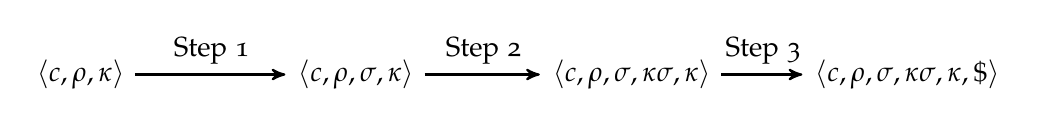
\begin{tikzpicture}[->,>=stealth',shorten >=1pt,auto,node distance=3.5cm,
  thick,main node/.style={font=\sffamily\bfseries}]

  \node[main node] (101) at (0, 1)
    {$\cek{c}{\rho}{\kappa}$};
  \node[main node] (102) [right of = 101]
    {$\cesk{c}{\rho}{\sigma}{\kappa}$};
  \node[main node] (103) [right of = 102]
    {$\cessk{c}{\rho}{\sigma}{\kappa\sigma}{\kappa}$};
  \node[main node] (104) [right of = 103]
    {$\cesskc{c}{\rho}{\sigma}{\kappa\sigma}{\kappa}{\$}$};

  \path[->]
    (101) edge node {Step 1} (102)
    (102) edge node {Step 2} (103)
    (103) edge node {Step 3} (104);

\end{tikzpicture}
\caption{An AAM-style approach for producing a pushdown abstract machine} \label{fig:M1}
\end{figure}

\subsection{A JavaScript Analysis in MAAM}

\js{} has a large, complex specification and many implementations which
practically define the expected semantics of \js{}. Rather than describe and
implement our own semantics, we implement the \lambdajs{} semantics as described
by Guha et. al. \cite{lambdajs}. Additionally, we reused their Haksell library
as our desugaring front-end.

\begin{figure}
\centering

\begin{lstlisting}
data Frame =
    LetK [(Name, Set AValue)] Name [(Name, TExp)] TExp
  | AppL [TExp]
  | AppR (Set AValue) [(Set AValue)] [TExp]
  | ObjK [(String, (Set AValue))] Name [(Name, TExp)]
    -- Array Dereferencing
  | FieldRefL TExp
  | FieldRefR (Set AValue)
    -- Array Assignment
  | FieldSetA TExp         TExp
  | FieldSetN (Set AValue) TExp
  | FieldSetV (Set AValue) (Set AValue)
    -- Property Deletion
  | DeleteL TExp
  | DeleteR (Set AValue)
    -- Fig 2. Mutable References
  | RefSetL TExp
  | RefSetR (Set AValue)
  | RefK
  | DeRefK
    -- Fig 8. Control Operators
  | IfK TExp TExp
  | SeqK TExp
  | WhileL TExp TExp
  | WhileR TExp TExp
  | LabelK Label
  | BreakK Label
  | TryCatchK TExp Name
  | TryFinallyL TExp
  | TryFinallyR (Set AValue)
  | ThrowK
    -- Fig 9. Primitive Operations
  | PrimOpK Op [(Set AValue)] [TExp]
  deriving (Eq, Ord)
instance PartialOrder Frame where pcompare = discreteOrder
\end{lstlisting}
\caption{The Frame, i.e., Continuation Datatype}
\end{figure}

\begin{figure}
\centering

\begin{lstlisting}
pushFrame :: (Analysis $\varsigma$ m) => Frame -> m ()
pushFrame fr = do
  fp  <- getL konL
  fp' <- nextFramePtr
  modifyL kstoreL (mapInsertWith (\/) fp' (singleton (fr, fp))
  putL konL fp'

popFrame :: (Analysis $\varsigma$ m) => m Frame
popFrame = do
  fp <- getL konL
  k$\sigma$ <- getL kstoreL
  (fr, fp') <- mset (mjoin (liftMaybeSet (k$\sigma$ # fp)))
  putL konL fp'
  return fr
\end{lstlisting}
\caption{Pushing and Popping Stack Frames}
\end{figure}

We reformulated the \lambdajs{} reduction semantics into a state machine
semantics with explicit continuations. The \lambdajs{} evaluation contexts
became our \emph{Frame} data type. Additionally, we do not divide the
evaluation contexts into two sets and use syntactic stepping rules to implement
exceptional control flow. We choose to implement exceptional control flow with
meta functions that crawl the stack looking for appropriate return points.

\section{Implementation}

Our static analysis system is the composition of significant existing work. This
exemplifies the ethos of \maam{}: implement only the semantics and derive
analyses for free. In particular, we have four primary components:

\begin{itemize}
\item The \lambdajs{} Parser \& Desugarer
\item The \lambdajs{} Standard Libarary
\item A \lambdajs{} State Machine with Explicit Continuations
\item The \maam{} Framework
\end{itemize}

The third item is the main contribution of this project.

\subsection{MAAM}

The \maam{} framework separates the semantics of a programming language from the
control flow. This same implementation of \lambdajs{} can be used with different
monads to produce path and flow sensitive analysis, as well as other kinds of
analysis. With an appropriate set of monads, traditional points-to constraints
could be generated. We note that we did not in the end implement each of these
analyses for \js{}, although we plan to do so in our continuation of this work.

\subsection{\lambdajs{} State Machine with Explicit Continuations}

We translated the deterministic, reduction semantics of \lambdajs{} directly
into a monadic state machine with explicit continuations. The reduction
semantics maps naturally to a state machine with explicit continuations. The
evaluation contexts become \emph{frames} and nested reduction contexts become a
list of frames.

Adapting the deterministic semantics to a monadic semantics consists primarily
of identifying control branching locations and inserting monadic splits at those
points. We do not insert monadic splits at value joins as this would result in
state space explosions. Inserting monadic splits only at control branches
enables the monad to control path and flow sensitivity.

We replaced substitution in the \lambdajs{} semantics with an
environment. Finally, we replaced the syntactic exception handling code with a
meta-function that searches the stack for the appropriate handler.

We found the entire translation process completely straightforward and
mechanical, albeit time consuming due to the size of \lambdajs{} and number of
primitive operations.

\begin{figure}
\centering


\begin{tikzpicture}[->,>=stealth',shorten >=1pt,auto,node distance=5cm,
  thick,main node/.style={font=\sffamily\bfseries}]

  \node[main node] (101) at (0, 1)
    {JS Code};
  \node[main node] (102) [right of = 101]
    {\lambdajs{} Code};
  \node[main node] (103) [right of = 102]
    {Analysis Results};

  \path[->]
    (101) edge node {Parse \& Desugar} (102)
    (102) edge node {\maam{} Analyzer} (103);

\end{tikzpicture}
\caption{The Architecture of Our Analysis System. The second arrow is original work.}
\end{figure}

\section{Related Work}
\subsection{The Essence of JavaScript: \lambdajs{}}

The \lambdajs{} work provides a complete, practical foundation to perform
research on real-world JavaScript programs. The \lambdajs{} work identifies a
simplified language that captures the essential features of \js{}. The
\lambdajs{} language is the composition of four distinct semantics: function and
object semantics, mutable references, prototypal inheritance, and control
operators. In the authors' experience, implementing this semantics is time
consuming, but mindless. The complexity of \js{} is not apparent in the
\lambdajs{} model.

The complexity of \js{} is fully captured by a desugaring phase which replaces
certain forms, such as \texttt{with}, with simpler \js{} code. Additionally, the
\lambdajs{} team has an implementation of the \js{} standard library which
abstracts away the details of string and number coercions. These coercions are
specified by many pages of non-trivial pseudo-code in the ECMAScript 3rd Edition
standard.

\section{Conclusion}



\bibliography{paper}{}
\bibliographystyle{acm}

\end{document}
